\chapter{Технологический раздел}


\section{Средства реализации}
\hspace{0.6cm} Для реализации программы были следующие языки программирования:
\begin{itemize}
	\item Python (v.3.9\cite{web:python}) для написания интерфейса программы и отрисовки рук. Python является простым в использовании средством для выполнения небольших задач, таких как чтение и запись, отрисовка оконного интерфейса;
	\item Prolog (SWI-Prolog\cite{web:prolog}) для написания функций проверки точек на корректность.
\end{itemize}
 
\section{Описание структуры базы знаний}

\subsection{Описание фактов}
\hspace{0.6cm} В данном разделе в листингах \ref{facts:fingermotiontype} - \ref{list:angledettype} описаны все факты и их назначения.
\subsubsection{finger\_motion\_type}
\hspace{0.6cm} Каждый палец (кроме большого) определяется 4 точками (3 точки для большого пальца), следовательно необходимо проверять 3 различных угла при сгибе пальцев (2 для большого), а также угол отклонения пальца при отведении пальца. Таким образом, каждому пальцу соответствует 4 типа проверок.

\begin{itemize}
	\item FingerType - тип пальца;
	\item AbductionType - тип сгиба, отведение или привидение;
	\item Flexion1 - обозначение, для определения места на пальце, в котором происходит сгиб.
\end{itemize}

\begin{lstlisting}[caption=Знания о типах проверок каждого пальца, label=facts:fingermotiontype]
%finger_motion_type(FingerType, AbductionType, Flexion1, Flexion2, Flexion3).

finger_motion_type(thumb, bpprived, bppsgib1, bppsgib2, bppsgib2).
finger_motion_type(index, oprived, o2sgib1, o2sgib2, o2sgib3).
finger_motion_type(middle, oprived, o3sgib1, o3sgib2, o3sgib3).
finger_motion_type(ring, oprived, o4sgib1, o4sgib2, o4sgib3).
finger_motion_type(little, oprived, o5sgib1, o5sgib2, o5sgib3).
\end{lstlisting}

\subsubsection{angle\_type\_limits}
\hspace{0.6cm} Каждому типу проверок соответствуют диапазоны углов, которые допустимы при том или ином движении пальца.

\begin{itemize}
	\item Finger - тип пальца;
	\item MinAngle - минимальное значение угла отклонения;
	\item MaxAngle - максимальное значение угла отклонения.
\end{itemize}

\begin{lstlisting}[caption=Знания об амплитудах углов, label=list:angle_limits]
%angle_type_limits(Finger, MinAngle, MaxAngle)

angle_type_limits(bpabc, -80, 80).
angle_type_limits(bpbcd, -50, 50).
angle_type_limits(bpcde, -90, 90).
angle_type_limits(oabc, -80, 80).
angle_type_limits(obcd, -100, 100).
angle_type_limits(ocde, -90, 90).
angle_type_limits(between, -30, 30).

angle_type_limits(bpprived, -50, 50).
angle_type_limits(oprived, -60, 60).
angle_type_limits(bppsgib1, -50, 50).
angle_type_limits(bppsgib2, -100, 80).

angle_type_limits(o2sgib1, -120, 90).
angle_type_limits(o2sgib2, -100, 100).
angle_type_limits(o2sgib3, -100, 100).

angle_type_limits(o3sgib1, -120, 90).
angle_type_limits(o3sgib2, -100, 100).
angle_type_limits(o3sgib3, -80, 80).

angle_type_limits(o4sgib1, -120, 90).
angle_type_limits(o4sgib2, -100, 100).
angle_type_limits(o4sgib3, -80, 80).

angle_type_limits(o5sgib1, -120, 90).
angle_type_limits(o5sgib2, -100, 100).
angle_type_limits(o5sgib3, -80, 80).

angle_type_limits(bppz, -100, 100).
\end{lstlisting}

\subsubsection{angle\_det\_type}
\hspace{0.6cm} Каждый из типов проверок отвечает за конкретную ось пространства, по которой проводится проверка.

\begin{itemize}
	\item Type - место сгиба на пальце;
	\item Axis - обозначает плоскость, в которой ищем угол.
\end{itemize}

\begin{lstlisting}[caption=Знания об осях типов проверок, label=list:angledettype]
%angle_det_type(Type, Axis)

angle_det_type(bpabc, all).
angle_det_type(bpbcd, all).
angle_det_type(bpcde, all).
angle_det_type(oabc, all).
angle_det_type(obcd, all).
angle_det_type(ocde, all).
angle_det_type(between, all).

angle_det_type(bpprived, x).
angle_det_type(oprived, x).
angle_det_type(bppsgib1, y).
angle_det_type(bppsgib2, y).

angle_det_type(o2sgib1, x).
angle_det_type(o2sgib2, x).
angle_det_type(o2sgib3, x).

angle_det_type(o3sgib1, x).
angle_det_type(o3sgib2, x).
angle_det_type(o3sgib3, x).

angle_det_type(o4sgib1, x).
angle_det_type(o4sgib2, x).
angle_det_type(o4sgib3, x).

angle_det_type(o5sgib1, x).
angle_det_type(o5sgib2, x).
angle_det_type(o5sgib3, x).

angle_det_type(bppz, z).
\end{lstlisting}

\subsection{Описание структур}
\hspace{0.6cm} Программой на Prolog для описания руки используются структуры Рука, Палец и Точка, описанные в листинге \ref{list:structures}.

\begin{itemize}
	\item point - структура Точка, состоит из трех координат;
	\item hand - структура Рука, из 5 Finger и двух опорных точек кисти;
	\item finger - структура Палец, состоит из 4 точек (3-х для большого пальца).
\end{itemize}
\begin{lstlisting}[caption=Структуры, label=list:structures]
point(X, Y, Z).

hand(
	finger(little, P0, P1, P2, P3),		%5|finger V
	finger(ring, P4, P5, P6, P7),		%4|finger IV
	finger(middle, P8, P9, P10, P11),	%3|finger III
	finger(index, P12, P13, P14, P15),	%2|finger II
	finger(thumb, P16, P17, P18),		%1|finger I
	P19, P20							
).	
\end{lstlisting}

\newpage

\subsection{Описание правил}
\hspace{0.6cm} В данном разделе в листингах \ref{rules:validangle} - \ref{rules:writepoints} описаны все правила, их назначение и использованные в них переменные.

\subsubsection{valid\_angle}
\hspace{0.6cm} valid\_angle - правило, с помощью которого определяется, входит ли данный угол в допустимый диапазон [MinAngle;MaxAngle]. Значения MinAngle и MaxAngle зависят от типа проверяемого угла.

\begin{itemize}
	\item Type - тип проверяемого угла;
	\item Angle - заданное значение угла;
	\item MinAngle - минимальный возможный угол;
	\item MaxAngle - максимальный возможный угол.
\end{itemize}

\begin{lstlisting}[caption=Реализация правила valid\_angle, label=rules:validangle]
valid_angle(Type, Angle):-
	angle_type_limits(Type, MinAngle, MaxAngle),
	MinAngle =< Angle, Angle =< MaxAngle.
\end{lstlisting}


\subsubsection{vec\_length}
\hspace{0.6cm} vec\_length - правило, которое определяет длину вектора.

\begin{itemize}
	\item vector(X,Y,Z) - структура <<вектор>>, определяемая тремя координатами;
	\item Len - длина вектора.
\end{itemize}

\begin{lstlisting}[caption=Реализация правила vec\_length, label=rules:veclength]
vec_length(vector(X, Y, Z), Len) :- Len is sqrt(X * X + Y * Y + Z * Z).
\end{lstlisting}

\subsubsection{vec\_length\_sqr}

\hspace{0.6cm} vec\_length\_sqr - правило, которое определяет квадрат длины вектора.

\begin{itemize}
	\item vector(X,Y,Z) - структура <<вектор>>, определяемая тремя координатами;
	\item Len - квадрат длины вектора.
\end{itemize}

\begin{lstlisting}[caption=Реализация правила vec\_length\_sqr, label=rules:veclengthsqr]
vec_length_sqr(vector(X, Y, Z), Len) :- Len is X * X + Y * Y + Z * Z.
\end{lstlisting}

\subsubsection{dot\_prod}
\hspace{0.6cm} dot\_prod - правило, которое получает две структуры vector и помещает в DotProd значение их произведения.

\begin{itemize}
	\item vector(X,Y,Z) - структура <<вектор>>, определяемая тремя координатами;
	\item DotProd - результат скалярного произведения векторов.
\end{itemize}

\begin{lstlisting}[caption=Реализация правила dot\_prod, label=rules:dotprod]
dot_prod(vector(X1, Y1, Z1), vector(X2, Y2, Z2), DotProd) :-
	DotProd is X1 * X2 + Y1 * Y2 + Z1 * Z2.
\end{lstlisting}

\subsubsection{rad\_to\_deg}
\hspace{0.6cm} rad\_to\_deg - правило, которое получает значение в радианах и переводит его в градусы.

\begin{itemize}
	\item Radian - величина угла в радианах;
	\item Degrees - величина угла в градусах.
\end{itemize}

\begin{lstlisting}[caption=Реализация правила rad\_to\_deg, label=rules:radtodeg]
rad_to_deg(Radian, Degrees) :- Degrees is Radian * 180 / 3.1415.
\end{lstlisting}
\subsubsection{deg\_to\_rad}
\hspace{0.6cm} deg\_to\_rad - правило, которое получает значение в градусах и переводит его в радианы.

\begin{itemize}
	\item Radian - величина угла в радианах;
	\item Degrees - величина угла в градусах.
\end{itemize}

\begin{lstlisting}[caption=Реализация правила deg\_to\_rad, label=rules:degtorad]
deg_to_rad(Degrees, Radian) :- Radian is Degrees * 3.1415 / 180.
\end{lstlisting}

\subsubsection{angle\_between\_vectors}
\hspace{0.6cm} angle\_between\_vectors - правило, которое определяет угол между двумя заданными векторами.

\begin{itemize}
	\item Vector1, Vector2 - структуры векторов, которые состоят из 3 переменных X,Y,Z;
	\item Angle - значение угла между векторами в градусах;
	\item Len1Sqr, Len2Sqr - значения квадратов длин Vector1 и Vector2 соответственно;
	\item DotProd - значение скалярного произведения векторов Vector1, Vector2;
	\item AngleRad - значение угла в радианах.
\end{itemize}

\begin{lstlisting}[caption=Реализация правила angle\_between\_vectors, label=rules:anglebetweenvectors]
angle_between_vectors(Vector1, Vector2, Angle) :-
	vec_length_sqr(Vector1, Len1Sqr),
	vec_length_sqr(Vector2, Len2Sqr),
	dot_prod(Vector1, Vector2, DotProd),
	AngleRad is acos(DotProd / sqrt(Len1Sqr * Len2Sqr)),
	rad_to_deg(AngleRad, Angle).
\end{lstlisting}

\subsubsection{get\_angle}
\hspace{0.6cm} get\_angle - правило, которое по заданным точкам в пространстве определяет угол между векторами, которые они образовывают.

\begin{itemize}
	\item all - обозначение того, что искать необходимо угол по всем осям сразу;
	\item x - обозначение того, что искать необходимо угол по оси Х;
	\item y - обозначение того, что искать необходимо угол по Y;
	\item z - обозначение того, что искать необходимо угол по Z;
	\item point(X, Y, Z) - структура, заданная тремя координатами;
	\item Angle - значение угла между векторами, образованными точками.
\end{itemize}

\begin{lstlisting}[caption=Реализация правила get\_angle, label=rules:getangle]
get_angle(all, point(X1, Y1, Z1), point(X2, Y2, Z2), point(X3, Y3, Z3), Angle) :-
	AX is X2 - X1, AY is Y2 - Y1, AZ is Z2 - Z1,
	BX is X3 - X2, BY is Y3 - Y2, BZ is Z3 - Z2,
	angle_between_vectors(vector(AX, AY, AZ), vector(BX, BY, BZ), Angle).
	
get_angle(x, point(X1, Y1, Z1), point(X2, Y2, Z2), point(X3, Y3, Z3), Angle) :-
	AY is Y1 - Y2, AZ is Z1 - Z2,
	BY is Y3 - Y2, BZ is Z3 - Z2,
	angle_between_vectors(vector(0, AY, AZ), vector(0, BY, BZ), Angle).
	
get_angle(y, point(X1, Y1, Z1), point(X2, Y2, Z2), point(X3, Y3, Z3), Angle) :-
	AX is X2 - X1, AZ is Z2 - Z1,
	BX is X3 - X2, BZ is Z3 - Z2,
	angle_between_vectors(vector(AX, 0, AZ), vector(BX, 0, BZ), Angle).
	
get_angle(z, point(X1, Y1, Z1), point(X2, Y2, Z2), point(X3, Y3, Z3), Angle) :-
	AX is X2 - X1, AY is Y2 - Y1,
	BX is X3 - X2, BY is Y3 - Y2,
	angle_between_vectors(vector(AX, AY, 0), vector(BX, BY, 0), Angle).
\end{lstlisting}


\subsubsection{validate\_angle}
\hspace{0.6cm} validate\_angle - правило, которое проверяет, является ли значение угла между векторами по заданным трём точкам допустимым для заданного типа угла.

\begin{itemize}
	\item Type - тип проверяемого угла;
	\item Point1, Point2, Point3 - структуры точек, заданных тремя координатами.
\end{itemize}

\begin{lstlisting}[caption=Реализация правила validate\_angle, label=rules:validateangle]
validate_angle(Type, Point1, Point2, Point3) :-
	hand:angle_det_type(Type, Axis),
	get_angle(Axis, Point1, Point2, Point3, Angle),
	write_files:write_angle(Type, Angle),
	hand:valid_angle(Type, Angle).
\end{lstlisting}

\subsubsection{validate\_points}
\hspace{0.6cm} validate\_points - процедура, которое проверяет корректность координат трёх точек по заданному типу угла. Состоит из трёх правил. Первое проверяет наличие и корректность координат, второе проверяет на корректность угол между тремя точками, а третье правило выводит сообщение о том, что точки не подходят, если угол не допустим.

\begin{itemize}
	\item Type -тип угла (между какими точками проверяется угол и какие заданы на него ограничения);
	\item X,Y,Z - список координат точки по X, Y, Z.
\end{itemize}

\begin{lstlisting}[caption=Реализация правила validate\_points, label=rules:validatepoints]
validate_points(Type, [X1, Y1, Z1], [X2, Y2, Z2], [X3, Y3, Z3]):-
	not(check_3coords([X1, Y1, Z1], [X2, Y2, Z2], [X3, Y3, Z3])),
	write_files:write_invalid_data().

validate_points(Type, [X1, Y1, Z1], [X2, Y2, Z2], [X3, Y3, Z3]):-
	check_3coords([X1, Y1, Z1], [X2, Y2, Z2], [X3, Y3, Z3]),
	validate_angle(Type, point(X1, Y1, Z1), point(X2, Y2, Z2), point(X3, Y3, Z3)),
	write_files:write_angle_is_valid(Type).
	
validate_points(Type, [X1, Y1, Z1], [X2, Y2, Z2], [X3, Y3, Z3]):-
	check_3coords([X1, Y1, Z1], [X2, Y2, Z2], [X3, Y3, Z3]),
	not(validate_angle(Type, point(X1, Y1, Z1), point(X2, Y2, Z2), point(X3, Y3, Z3))),
	write_files:write_invalid_points([X1, Y1, Z1], [X2, Y2, Z2], [X3, Y3, Z3]).
\end{lstlisting}

\subsubsection{validate\_hand}
\hspace{0.6cm} validate\_hand - правило, которое проверяет переданные ему конструкции finger.

\begin{itemize}
	\item hand - структура <<Рука>>, которая состоит из 5 структур типа Finger, которые состоят из 4 точек для указательного, среднего, безымянного и мизинца, из 3-х точек для большего пальца, а также оставшихся двух ключевых точек на ладони: пясть и запястье;
	\item finger - структура пальца, состоящая из 3 или 4 точек;
	\item Wrist - точка на запястье;
	\item p19 - точка на пясти.
\end{itemize}

\begin{lstlisting}[caption=Реализация правила validate\_hand, label=rules:validatehand]
validate_hand(hand:hand(Finger5, Finger4, Finger3, Finger2, Finger1, P19, Wrist)):-
	validate_finger(Finger5, P19, Wrist),
	validate_finger(Finger4, P19, Wrist),
	validate_finger(Finger3, P19, Wrist),
	validate_finger(Finger2, P19, Wrist),
	validate_finger(Finger1, P19, Wrist).
\end{lstlisting}

\subsubsection{validate\_finger}
\hspace{0.6cm} validate\_finger - правило, которое проверяет корректность точек на пальце. .

\begin{itemize}
	\item finger - структура пальца, которая состоит из вида пальца (большой/безымянный/средний и т. д.) и точек-концов фаланг;
	\item Wrist - точка на запястье;
	\item p19 - точка на пясти;
	\item finger\_motion\_type - знание об амплитуде угла для конкретного типа пальца.
\end{itemize}

\begin{lstlisting}[caption=Реализация правила validate\_finger, label=rules:validatefinger]
validate_finger(finger(thumb, P1, P2, P3), P19, Wrist):-
	finger_motion_type(thumb, Abduction, Flex1, Flex2, _),
	validate_points(bpabc, P1, P2, P3),
	validate_points(Abduction, P3, P2, Wrist),
	validate_points(Flex1, P1, P2, P3),
	validate_points(Flex2, P1, P2, Wrist),
	validate_points(bppz, P1, P2, P3).
\end{lstlisting}

\subsubsection{check\_coords}
\hspace{0.6cm} check\_coords - правило, которое проверяет наличие и валидность данных о координатах.

\begin{itemize}
	\item [X, Y, Z] - список координат.
\end{itemize}

\begin{lstlisting}[caption=Реализация правила check\_coords, label=rules:checkcoords]
check_coords([X, Y, Z]):- number(X), number(Y), number(Z).
\end{lstlisting}

\subsubsection{check\_3coords}
\hspace{0.6cm} check\_3coords - правило, которое проверяет наличие и валидность данных о координатах трёх точек.

\begin{itemize}
	\item [X1, Y1, Z1], [X2, Y2, Z2], [X3, Y3, Z3] - списки координат.
\end{itemize}

\begin{lstlisting}[caption=Реализация правила check\_3coords, label=rules:check3coords]
check_3coords([X1, Y1, Z1], [X2, Y2, Z2], [X3, Y3, Z3]) :-
	check_coords([X1, Y1, Z1]),
	check_coords([X2, Y2, Z2]),
	check_coords([X3, Y3, Z3]).
\end{lstlisting}

\subsubsection{validate\_all}
\hspace{0.6cm} validate\_all - правило, определяющее корректность точек двух рук. <<Входное>> правило программе.

\begin{itemize}
	\item Working\_Dir - путь к рабочей директории с файлом с координатами точек;
	\item Result - результат работы правила;
	\item Point1 - структура <<Точка>>, состоящая из трех координат.
\end{itemize}

\begin{lstlisting}[caption=Реализация правила validate\_all, label=rules:validateall]
validate_all(Working_Dir, Result,
	Point1, Point2, Point3, Point4, Point5, Point6, Point7,
	Point8, Point9, Point10, Point11, Point12, Point13, Point14,
	Point15, Point16, Point17, Point18, Point19, Point20, Point21,
	Point22, Point23, Point24, Point25, Point26, Point27, Point28,
	Point29, Point30, Point31, Point32, Point33, Point34, Point35,
	Point36, Point37, Point38, Point39, Point40, Point41, Point42
) :-
	working_directory(_, Working_Dir),
	open('points.txt', write, Stream),
	open('angles.txt', write, Stream2),
	close(Stream2),
	close(Stream),
	(	
		(
			validate_hand(
				hand:hand(
					finger(little, Point1, Point2, Point3, Point4),
					finger(ring, Point5, Point6, Point7, Point8),
					finger(middle, Point9, Point10, Point11, Point12),
					finger(index, Point13, Point14, Point15, Point16),
					finger(thumb, Point17, Point18, Point19),
					Point20, Point21
				)
			),
			validate_hand(
				hand:hand(
					finger(little, Point37, Point38, Point39, Point40),
					finger(ring, Point33, Point34, Point35, Point36),
					finger(middle, Point29, Point30, Point31, Point32),
					finger(index, Point25, Point26, Point27, Point28),
					finger(thumb, Point22, Point23, Point24),
					Point41, Point42
				)
			)
		)-> Result = "Ok"; Result = "Not"
	).
\end{lstlisting}

\subsubsection{write\_invalid\_data}
\hspace{0.6cm} write\_invalid\_data - правило, которое выводит сообщение о некорректности данных.

\begin{lstlisting}[caption=Реализация правила write\_invalid\_data, label=rules:writeinvaliddata]
write_invalid_data() :- write("Invalid data "), nl.
\end{lstlisting}

\subsubsection{write\_angle}
\hspace{0.6cm} write\_angle - правило, которое выводит значение угла.

\begin{itemize}
	\item Angle - значение угла.
\end{itemize}

\begin{lstlisting}[caption=Реализация правила write\_angle, label=rules:writeangle]
write_angle(Angle) :- write("Angle is "), write(Angle), nl.
\end{lstlisting}

\subsubsection{write\_angle}
\hspace{0.6cm} write\_angle - правило, которое выводит значение и тип угла.

\begin{itemize}
	\item Angle - значение угла;
	\item Type - тип угла.
\end{itemize}

\begin{lstlisting}[caption=Реализация правила write\_angle, label=rules:writeangle]
write_angle(Type, Angle):- write(Type), write(" angle is "), write(Angle), nl.
\end{lstlisting}

\subsubsection{write\_angle\_is\_valid}
\hspace{0.6cm} write\_angle\_is\_valid - правило, которое пишет о корректности угла в файл.

\begin{itemize}
	\item Type - тип данного угла.
\end{itemize}

\begin{lstlisting}[caption=Реализация правила write\_angle\_is\_valid, label=rules:writeangleisvalid]
write_angle_is_valid(Type) :- 
	open('angles.txt', append, Stream2),
	string_concat(Type, " is ok", Msg),
	write(Stream2, Msg), nl(Stream2),
	close(Stream2).
\end{lstlisting}

\subsubsection{write\_invalid\_points}
\hspace{0.6cm} write\_invalid\_points - правило, которое записывает некорректные точки в файл.

\begin{itemize}
	\item Point - структура точки, состоит из трех координат.
\end{itemize}

\begin{lstlisting}[caption=Реализация правила write\_invalid\_points, label=rules:writeinvalidpoints]
write_invalid_points(Point1, Point2, Point3) :-
	open('points.txt', append, Stream),
	write(Stream, [Point1, Point2, Point3]), nl(Stream),
	close(Stream).
\end{lstlisting}

\subsubsection{point\_to\_str}
\hspace{0.6cm} point\_to\_str - правило, которое приводит значение точки к строковому представлению.

\begin{itemize}
	\item Point - структура <<Точка>>, состоящая из трех координат;
	\item Str - строковое представление точки.
\end{itemize}

\begin{lstlisting}[caption=Реализация правила point\_to\_str, label=rules:pointtostr]
point_to_str(Point, Str) :-
	determ:get_coords(Point, X, Y, Z),
	number_string(X, StrX),
	number_string(Y, StrY),
	number_string(Z, StrZ),
	string_concat(StrX, ";", StrX1),
	string_concat(StrY, ";", StrY1),
	string_concat(StrX1, StrY1, StrXY),
	string_concat(StrXY, StrZ, StrXYZ),
	string_concat(StrXYZ, "\n", Str).
\end{lstlisting}

\subsubsection{write\_list}
\hspace{0.6cm} write\_list - правило, которое пишет в список в файл.

\begin{itemize}
	\item Stream - поток записи;
	\item \[\] - список;
	\item Head - голова списка;
	\item Tail - хвост списка.
\end{itemize}

\begin{lstlisting}[caption=Реализация правила write\_list, label=rules:writelist]
write_list(Stream, []).
write_list(Stream, [Head|Tail]) :-
	write(Stream, Head),
	write_list(Stream, Tail).
\end{lstlisting}

\subsubsection{write\_points} 
\hspace{0.6cm} write\_points - правило, которое пишет точки из списка в файл.

\begin{itemize}
	\item Filename - путь к файлу с координатами;
	\item PList - список координат, полученных из файлов.
\end{itemize}

\begin{lstlisting}[caption=Реализация правила write\_points, label=rules:writepoints]
write_points(PList,Filename) :-
    open(Filename, write, Stream),
    convlist(point_to_str, PList, StrList),
	write_list(Stream, StrList),
    close(Stream).
\end{lstlisting}

\section{Средства взаимодействия python и Prolog}

\hspace{0.6cm} Для обеспечения взаимодействия частей программы на языках Python и Prolog, была использована библиотека PySwip, которая позволяет делать запросы со входными данными из части Python, а также консультировать выбранные файлы. В листинге \ref{rules:PythonProlog} продемонстрированы две функции, использующиеся для взаимодействия.

\begin{lstlisting}[caption=Взаимодействие python и Prolog, label=rules:PythonProlog]
from pyswip import Prolog
import os

def append_base_stored(prolog, filename, filepath=None):
    if filepath is None:
        filepath = ''    
    fullpath = os.path.join(filepath, filename)
    prolog.consult(fullpath)
    
def get_answer(basestored, statement, filepath=None):
    prolog = Prolog()
    append_base_stored(prolog=prolog, 
                       filename=basestored,
                       filepath=filepath)
    return prolog.query(statement)

\end{lstlisting}

\hspace{0.6cm} append\_base\_stored - функция, которая по пути и имени файла консультирует файл по этому пути, тем самым запуская реализацию части программы на Prolog.

\hspace{0.6cm} get\_answer - функция, которая отправляет в программу запрос и возвращает состояние после того, как она обработала запрос.

\section{Интерфейс программы}
\hspace{0.6cm} Для удобства создания GUI для работы с кистями была выбрана библиотека tkinter, с надстройками позволяющими рисовать 3D изображения, а также добавить интерфейс взаимодействия с точками кисти, возможностью их изменять, сохранять или записывать в файл.

\hspace{0.6cm} Интерфейс на tkinter состоит из:
\begin{itemize}
	\item холста, на котором происходит отрисовка;
	\item небольшом изображении в углу экрана, которое служит для выбора точек на кисти, координаты которых пользователь может поменять;
	\item кнопок изменения координат выбранной точки по X, Y, Z;
	\item кнопок для загрузки и сохранения координат в файл;
	\item кнопки для проверки текущих точек на корректность.
\end{itemize}

\begin{figure}[ht!]
	\centering
	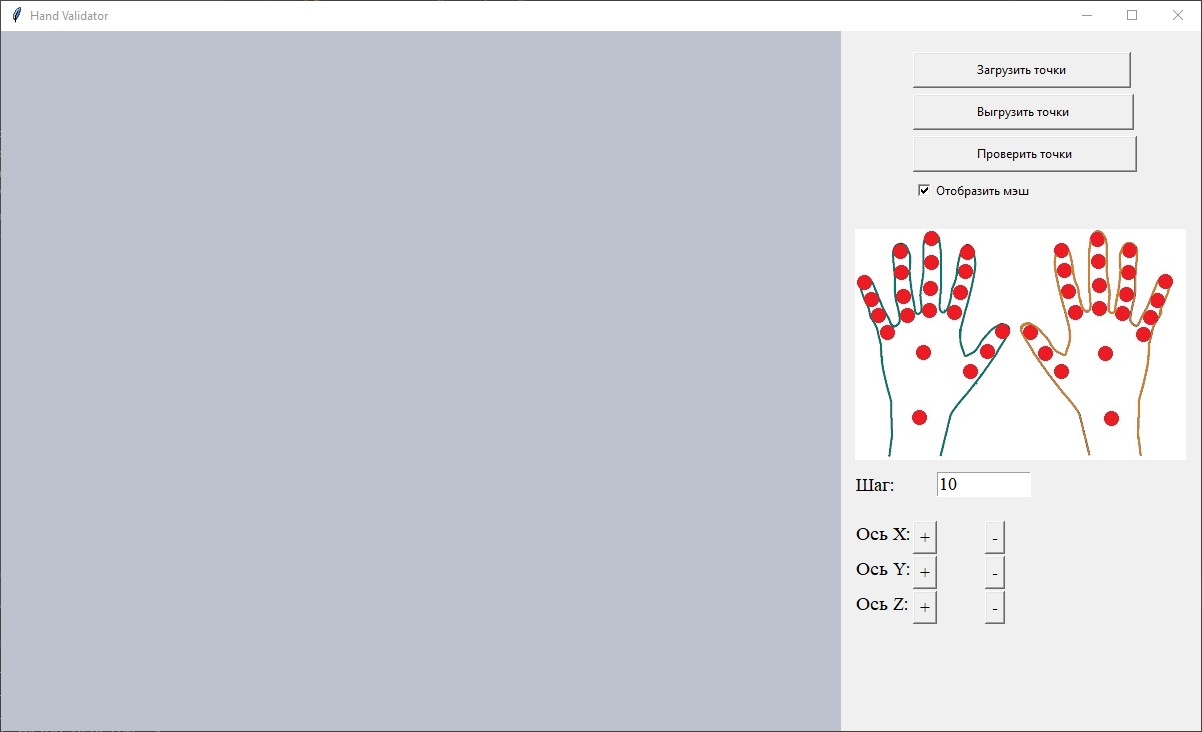
\includegraphics[scale=0.5]{example_gui.jpg}
	\caption{Интерфейс программы}
	\label{fig:gui}
\end{figure}

\section{Отрисовка рук в Python}

\hspace{0.6cm} Отрисовка кисти совершается следующим образом. Точки загружаются из текстового файла, которых должно быть 42. Полученные 42 точки делятся по 21, для каждой кисти соотвественно. После необходимых проверок на Prolog, по этим точкам рисуется каркас, показывающий их схематичное расположение относительно друг друга. При этом если ребра окрашены красным цветом, то это означает, что положение отдельной части руки в этих трех точках недопустимо. Левая рука окрашена зелёным цветом, а правая - рыжим. Точки обозначены чёрными квадратами.

\hspace{0.6cm} Чтобы визуально было проще понимать, какая рука где находится, а также определять, куда "смотрит" ладонь, а где ее тыльная сторона, было решено добавить модель кисти.

\hspace{0.6cm} Относительно каждых групп точек рисуется геометрическая фигура, отдаленно напоминающая ту часть кисти, которой соответствует. Каждая фаланга представляется призмой с основанием в форме треугольника, причём окончание пальца имеет треугольник меньшего размера.

\begin{itemize}
	\item class PhalanxModel - класс, определяющий структуру данных точек фаланги пальца и порядок её отображения;
	\item class EndPhalanxModel - класс, определяющий структуру данных точек конечной фаланги пальца и порядок её отображения, является наследником класса PhalanxModel, отличается от базового класса меньшим размером конечного треугольника-основания;
	\item class FingerModel - класс, определяющий структуру данных точек пальца и порядок его отображения;
	\item class HandModel - класс, определяющий структуру данных точек руки и порядок её отображения;
	\item class RightHandModel - класс, определяющий структуру данных точек правой руки и порядок отображения её, является наследником класса HandModel, отличается от базового класса другой последовательностью подаваемых координат для составления структуры.
\end{itemize}

\hspace{0.6cm} Перемещать камеру возможно с помощью стрелок на клавиатуре, масштабирование осуществляется с помощью кнопок '+' и '-'.

\section{Примеры работы}

\begin{figure}[ht!]
	\centering
	\includegraphics[scale=0.5]{example1.jpg}
	\caption{Пример работы с корректным расположением точек}
	\label{fig:example1}
\end{figure}

\begin{figure}[ht!]
	\centering
	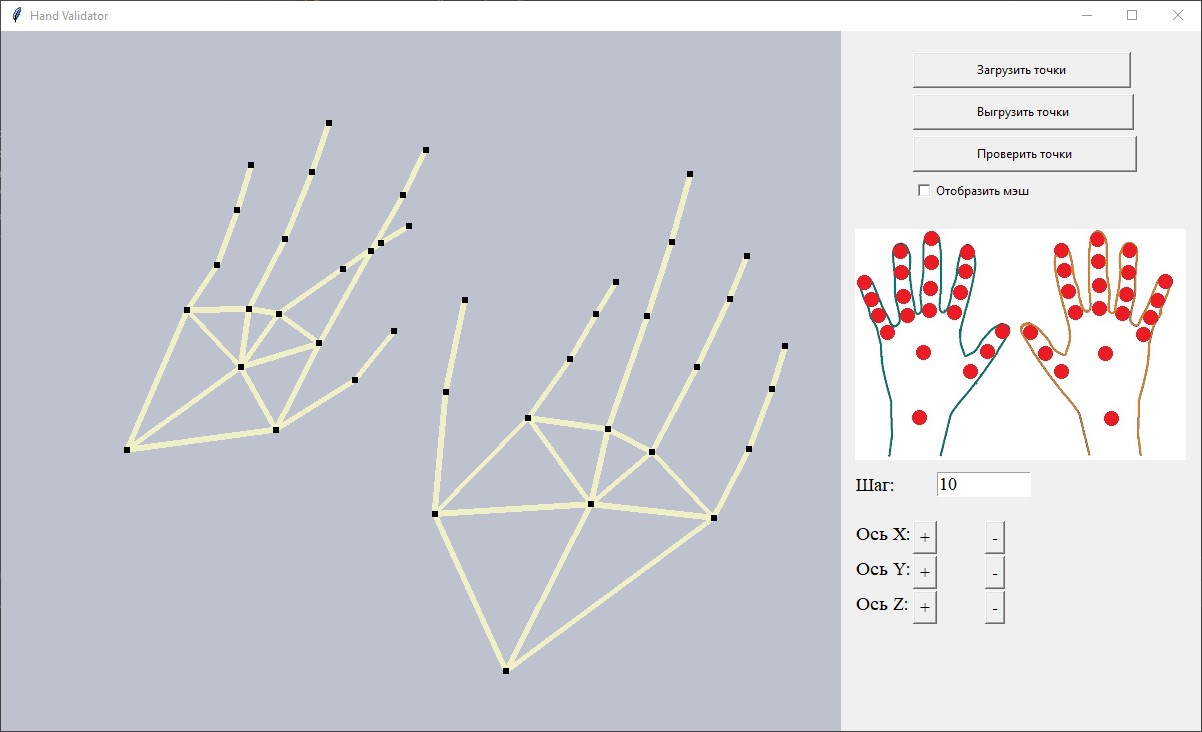
\includegraphics[scale=0.5]{example2.jpg}
	\caption{Пример работы только с каркасом}
	\label{fig:example2}
\end{figure}

\begin{figure}[ht!]
	\centering
	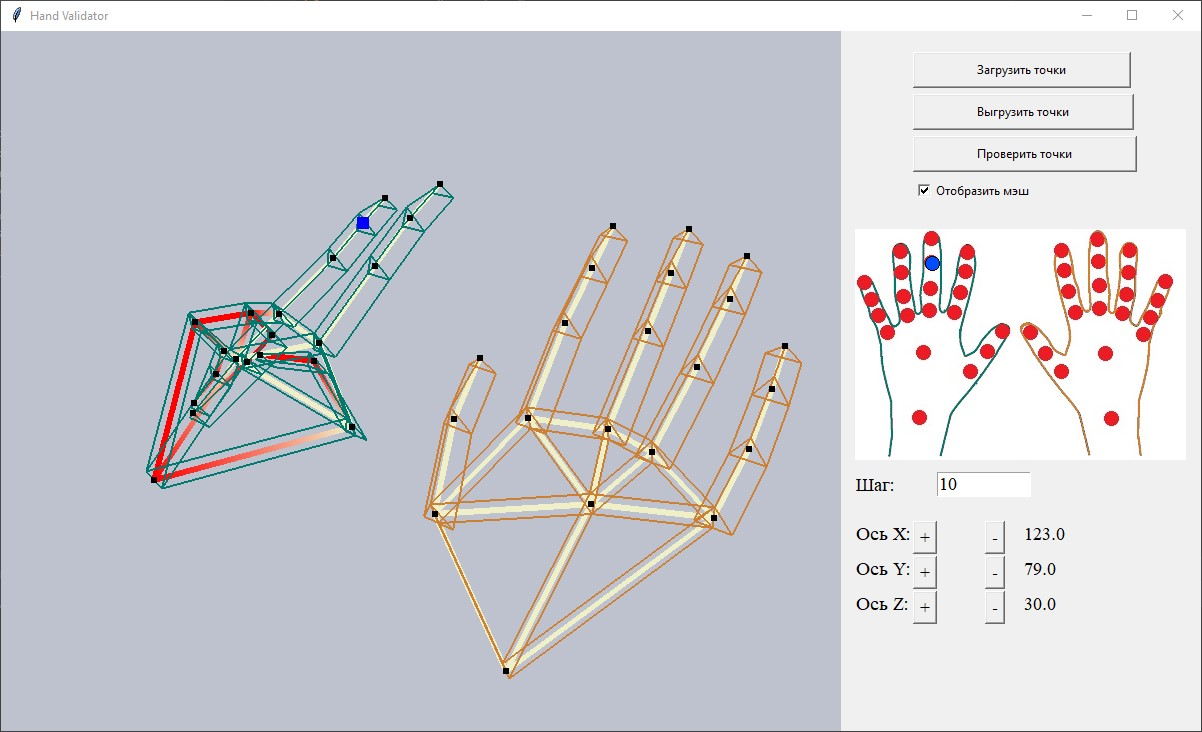
\includegraphics[scale=0.5]{example3.jpg}
	\caption{Пример работы с некорректным расположением точек}
	\label{fig:example3}
\end{figure}



